\chapter{Translations et Rotations}\label{ChTranslationsRotations}

\vspace{5cm}

\begin{acquis}
\begin{itemize}
\item tracer l’image d’une  figure par une translation;
\columnbreak
\item tracer l'image d'une figure par une rotation d'angle 45 ou 90°.
\end{itemize}
\end{acquis}


\activites

\begin{activite}[Un pas de côté]

Cinq élèves ont construit une image du danseur, en effectuant chacun une translation différente :
\begin{enumerate}
 \item Sarah, de 5 cm dans la direction de $d$ ;
 \item Vincent, horizontalement, vers la droite ;
 \item Mélanie, selon le vecteur $\vec{c}$ ;
 \item Juan, en la glissant de 3 cm ;
 \item Madina, en la déplaçant de 4 cm, vers la gauche et dans la direction de $b$.
 \end{enumerate}
 \begin{minipage}[c]{0.58\linewidth}
  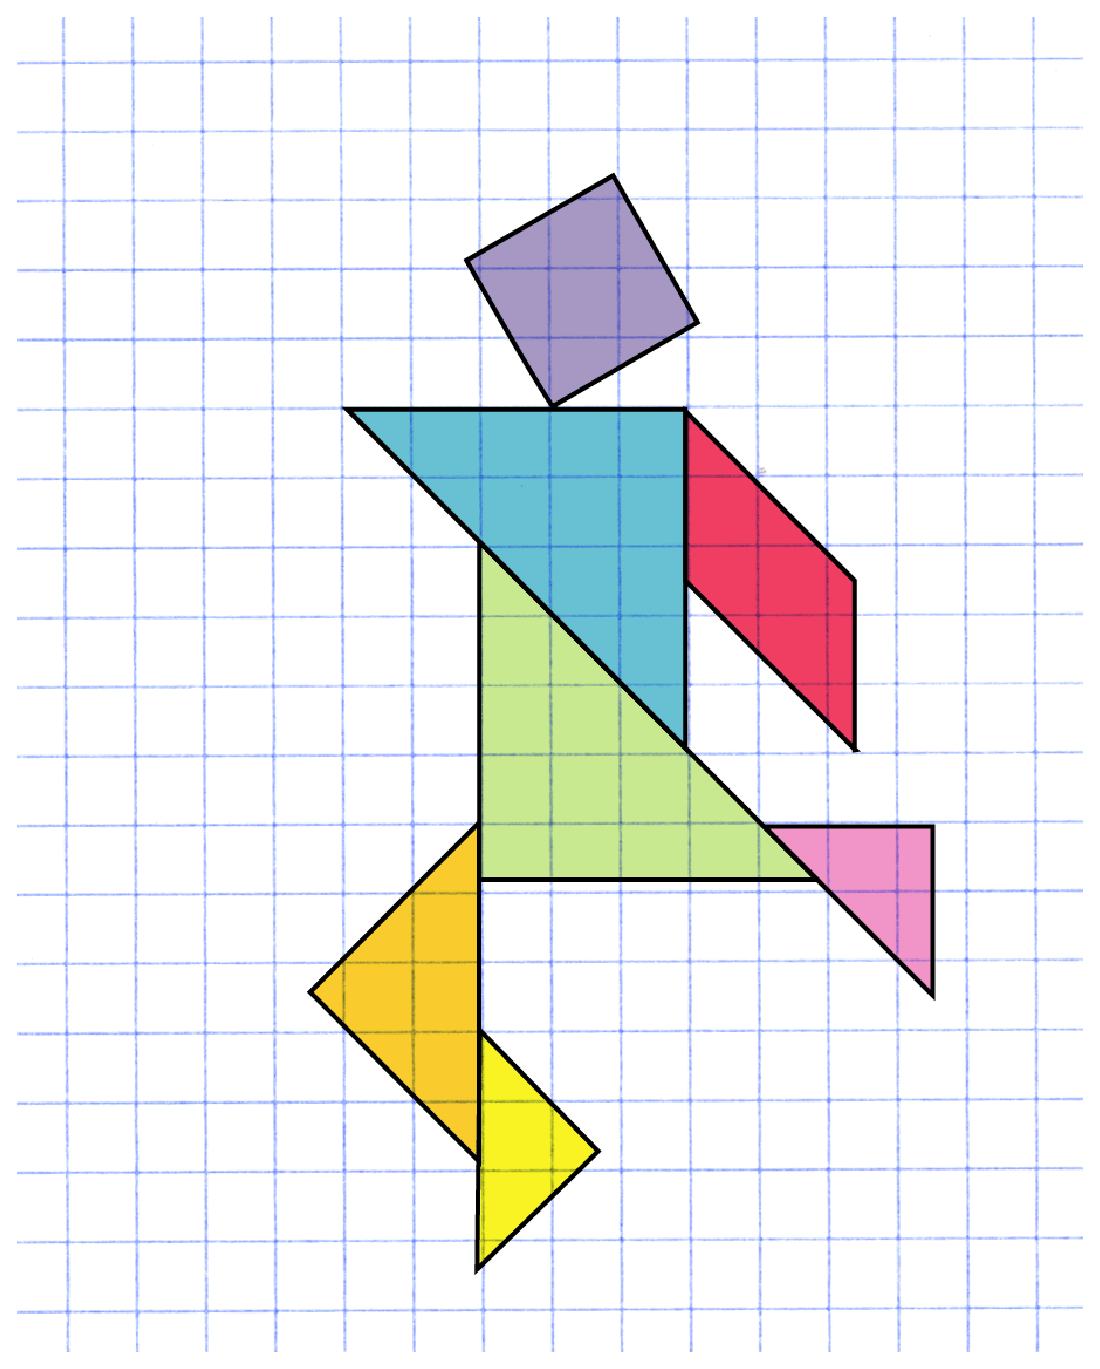
\includegraphics[width=8.4cm]{grille_danseur} 
  \end{minipage} \hfill%
  \begin{minipage}[c]{0.28\linewidth}
  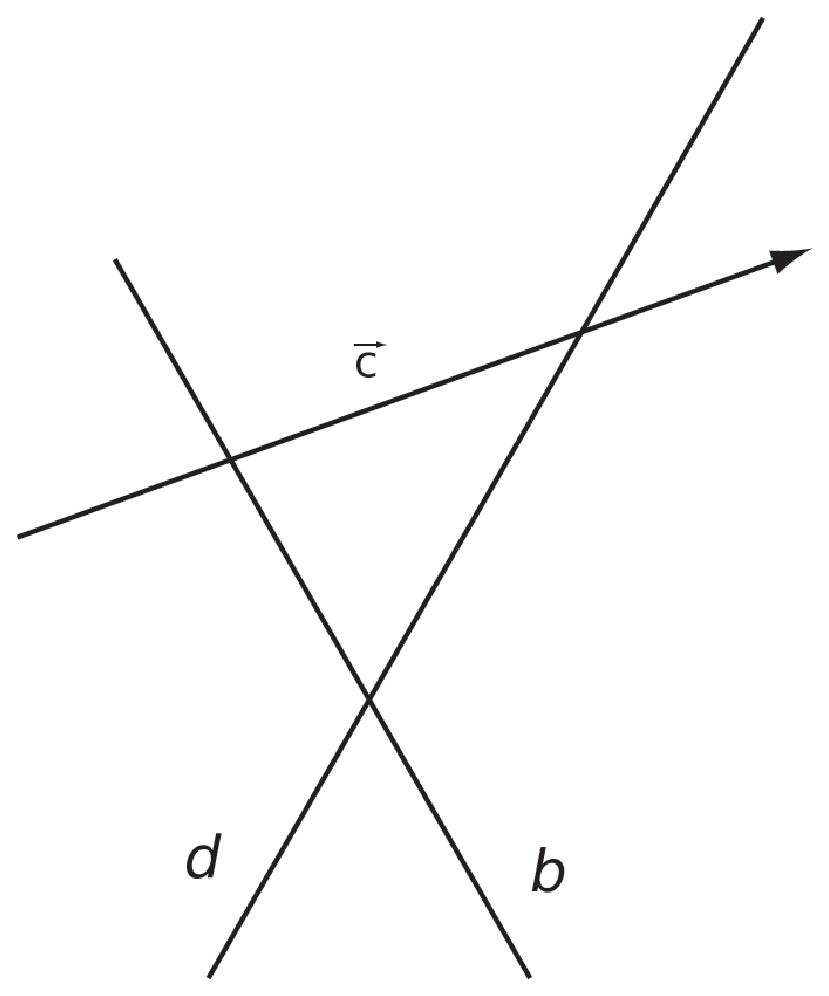
\includegraphics[width=4.2cm]{vecC_db}
  \end{minipage} \\
À l'aide des carreaux, construis ces cinq figures et compare tes résultats avec ceux de tes camarades.

\end{activite}

%%%%%%%%%%%%%%%%%%%%%%%%%%%%%%%%%%%%%%%%%%%%%%%%%%%%%%%%%%%%%%%%%%%%%%

%%%%%%%%%%%%%%%%%%%%%%%%%%%%%%%%%%%
%%%%%%%%%%%%%%%%%%%%%%%%%%%%%%%%%%%
%MiseEnPage
%%%%%%%%%%%%%%%%%%%%%%%%%%%%%%%%%%%
\newpage
%%%%%%%%%%%%%%%%%%%%%%%%%%%%%%%%%%%
%%%%%%%%%%%%%%%%%%%%%%%%%%%%%%%%%%%

\begin{activite}[Avoir du bons sens]

Voici une vingtaine de flèches représentant des vecteurs :
\begin{center} 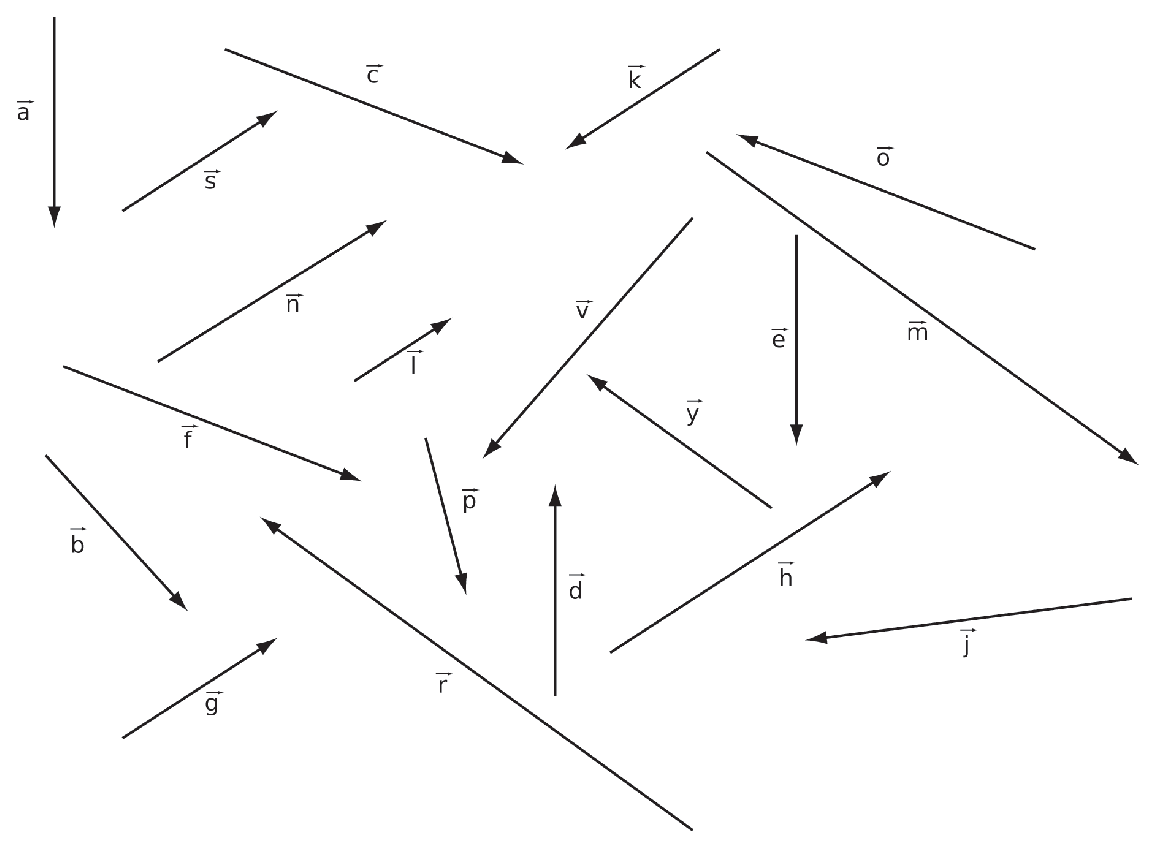
\includegraphics[width=16cm]{fleches_vecteurs}\end{center}

\begin{partie}[Classification]
Recopie puis complète le tableau en donnant tous les vecteurs possibles pour chaque question. Arrondis au dixième le plus proche tes mesures.
\begin{center}
 \renewcommand*\tabularxcolumn[1]{>{\centering\arraybackslash}m{#1}}
 \begin{ttableau}{0.9\linewidth}{4}
 \hline
 \rowcolor{A3}Vecteur & Même longueur que le vecteur & Même direction que le vecteur & Égal au vecteur \\\hline
 \rowcolor{F3} $\vec{a}$ & & & \\\hline
 \rowcolor{F3} $\vec{c}$ & & & \\\hline
 \rowcolor{F3} $\vec{q}$ & & & \\\hline
 \rowcolor{F3} $\vec{r}$ & & & \\\hline
 \end{ttableau}
 \end{center}
\end{partie}

\vspace{1em}

\begin{partie}[Qu'en penses-tu ?]
Détermine si les affirmations des élèves sont correctes ou non :
\begin{enumerate}
 \item Aline dit que le vecteur $\vec{c}$ est égal à deux fois le vecteur $\vec{a}$ ;
 \item Simon dit que le vecteur $\vec{d}$ est l'opposé du vecteur $\vec{e}$ ;
 \item Justine prétend que le vecteur $\vec{b}$ et $\vec{f}$ ont la même direction ;
 \item Mohamed dit que les vecteurs $\vec{c}$ et $\vec{j}$ ont la même intensité.
 \end{enumerate}
\end{partie}

\end{activite}

%%%%%%%%%%%%%%%%%%%%%%%%%%%%%%%%%%%%%%%%%%%%%%%%%%%%%%%%%%%%%%%%%%%%%%

\begin{activite}[Tourner dans tous les sens]

\begin{partie}[Dans quel sens]
 \begin{minipage}[c]{0.68\linewidth}
La figure ci-contre illustre une montre possédant qu'une seule aiguille.
\begin{enumerate}
 \item Reproduis le dessin puis dessine l'aiguille quand elle aura tourné de $90^\circ$ par rapport au centre $O$ ;
 \item Dessine l'aiguille quand elle aura tourné de $- 120^\circ$ par rapport au centre $O$.
 \end{enumerate}
  \end{minipage} \hfill%
  \begin{minipage}[c]{0.28\linewidth}
  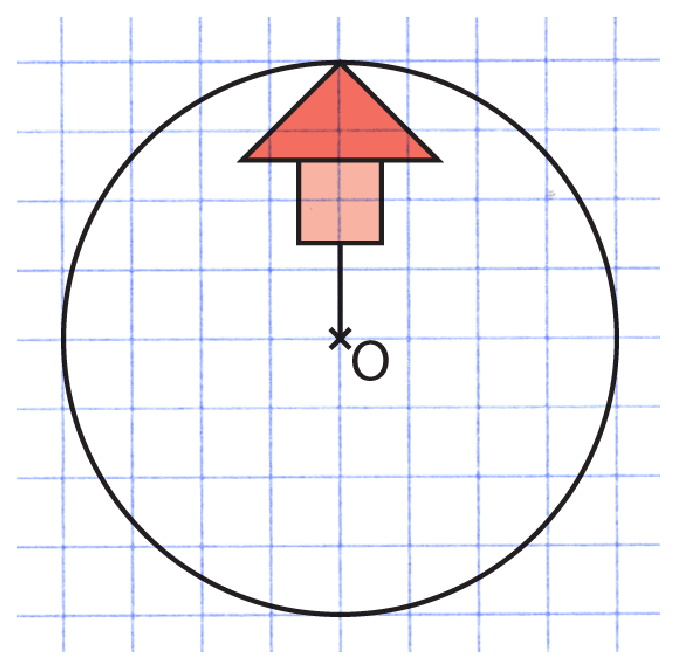
\includegraphics[width=4cm]{une_aiguille}
  \end{minipage} \\ 
\end{partie}

\begin{partie}[Le virage]
 \begin{minipage}[c]{0.50\linewidth}
Ci-contre une partie du circuit de Catalogne où la formule 1 vient d'entamer son virage.
\begin{enumerate}
 \item À l'aide d'un papier calque reproduit cette figure et dessine la voiture après qu'elle ait effectué une rotation de $80^\circ$ par rapport au centre $P$.
 \item Peut-on effectuer tout le virage en gardant le même rayon de rotation ?
 \end{enumerate}
  \end{minipage} \hfill%
  \begin{minipage}[c]{0.46\linewidth}
  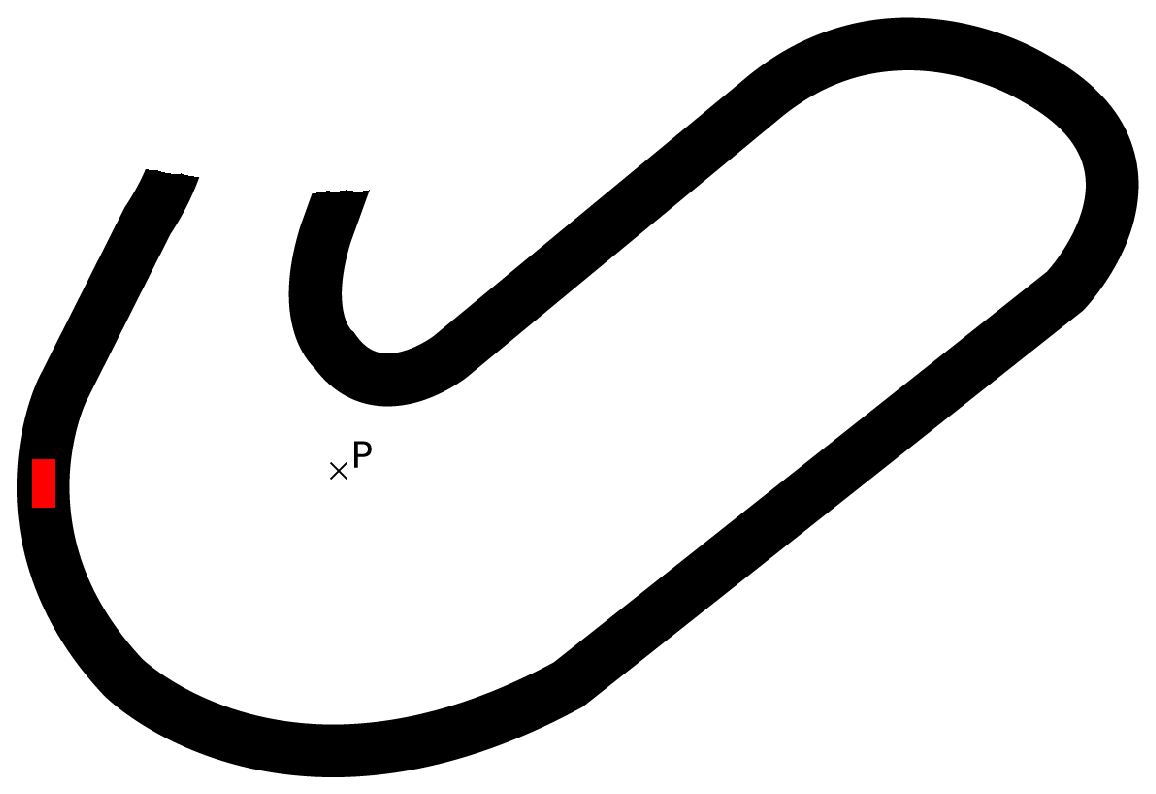
\includegraphics[width=6.9cm]{formule1_Catalogne}
  \end{minipage} \\ 
\end{partie}

\begin{partie}[Trouver le centre]
\vspace{.5em}
 \begin{minipage}[c]{0.28\linewidth}
  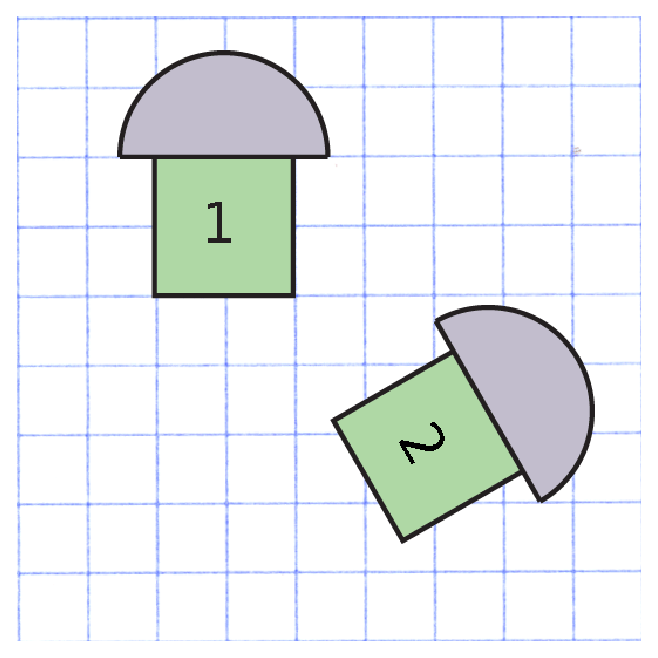
\includegraphics[width=4.7cm]{champi_rotation}
  \end{minipage} \hfill%
  \begin{minipage}[c]{0.58\linewidth}
Alice sait que la figure 2 a été obtenue après une rotation de la figure 1. \\[0.5em]
Pascal aimerait savoir où se trouve le centre de la rotation ainsi que l'angle de rotation. \\[0.5em]
Aline propose de tracer les médiatrices des segments reliant les sommets de la figure 1 aux sommets correspondants de la figure 2.
  \end{minipage} \\
\begin{enumerate}
 \item Recopie la figure puis effectue ce qu'Aline propose.
 \item Que remarques-tu ?
 \item Détermine où se trouve le centre ainsi que l'angle de la rotation qui permet de passer de la figure 1 à la figure 2.
 \end{enumerate}
\end{partie}

\end{activite}

%%%%%%%%%%%%%%%%%%%%%%%%%%%%%%%%%%%%%%%%%%%%%%%%%%%%%%%%%%%%%%%%%%%%%%


\cours
%\section{Une section}

% remarque : pour qu'un mot se retrouve dans le lexique : \MotDefinition{asymptote horizontale}{} 

\begin{aconnaitre}
Une \MotDefinition{translation}{} consiste à faire glisser une figure selon un \MotDefinition{vecteur}{} donné.\\[0.5em]
\begin{minipage}[c]{0.62\linewidth}
Un \textbf{vecteur} est représenté par une flèche et est défini par :
\begin{itemize}
 \item une direction (c'est la direction de la droite)
 \item un sens (c'est le sens de la flèche)
 \item une longueur (c'est la longueur du segment)
 \end{itemize}
 \end{minipage} \hfill%
 \begin{minipage}[c]{0.34\linewidth}
 \begin{center}
 %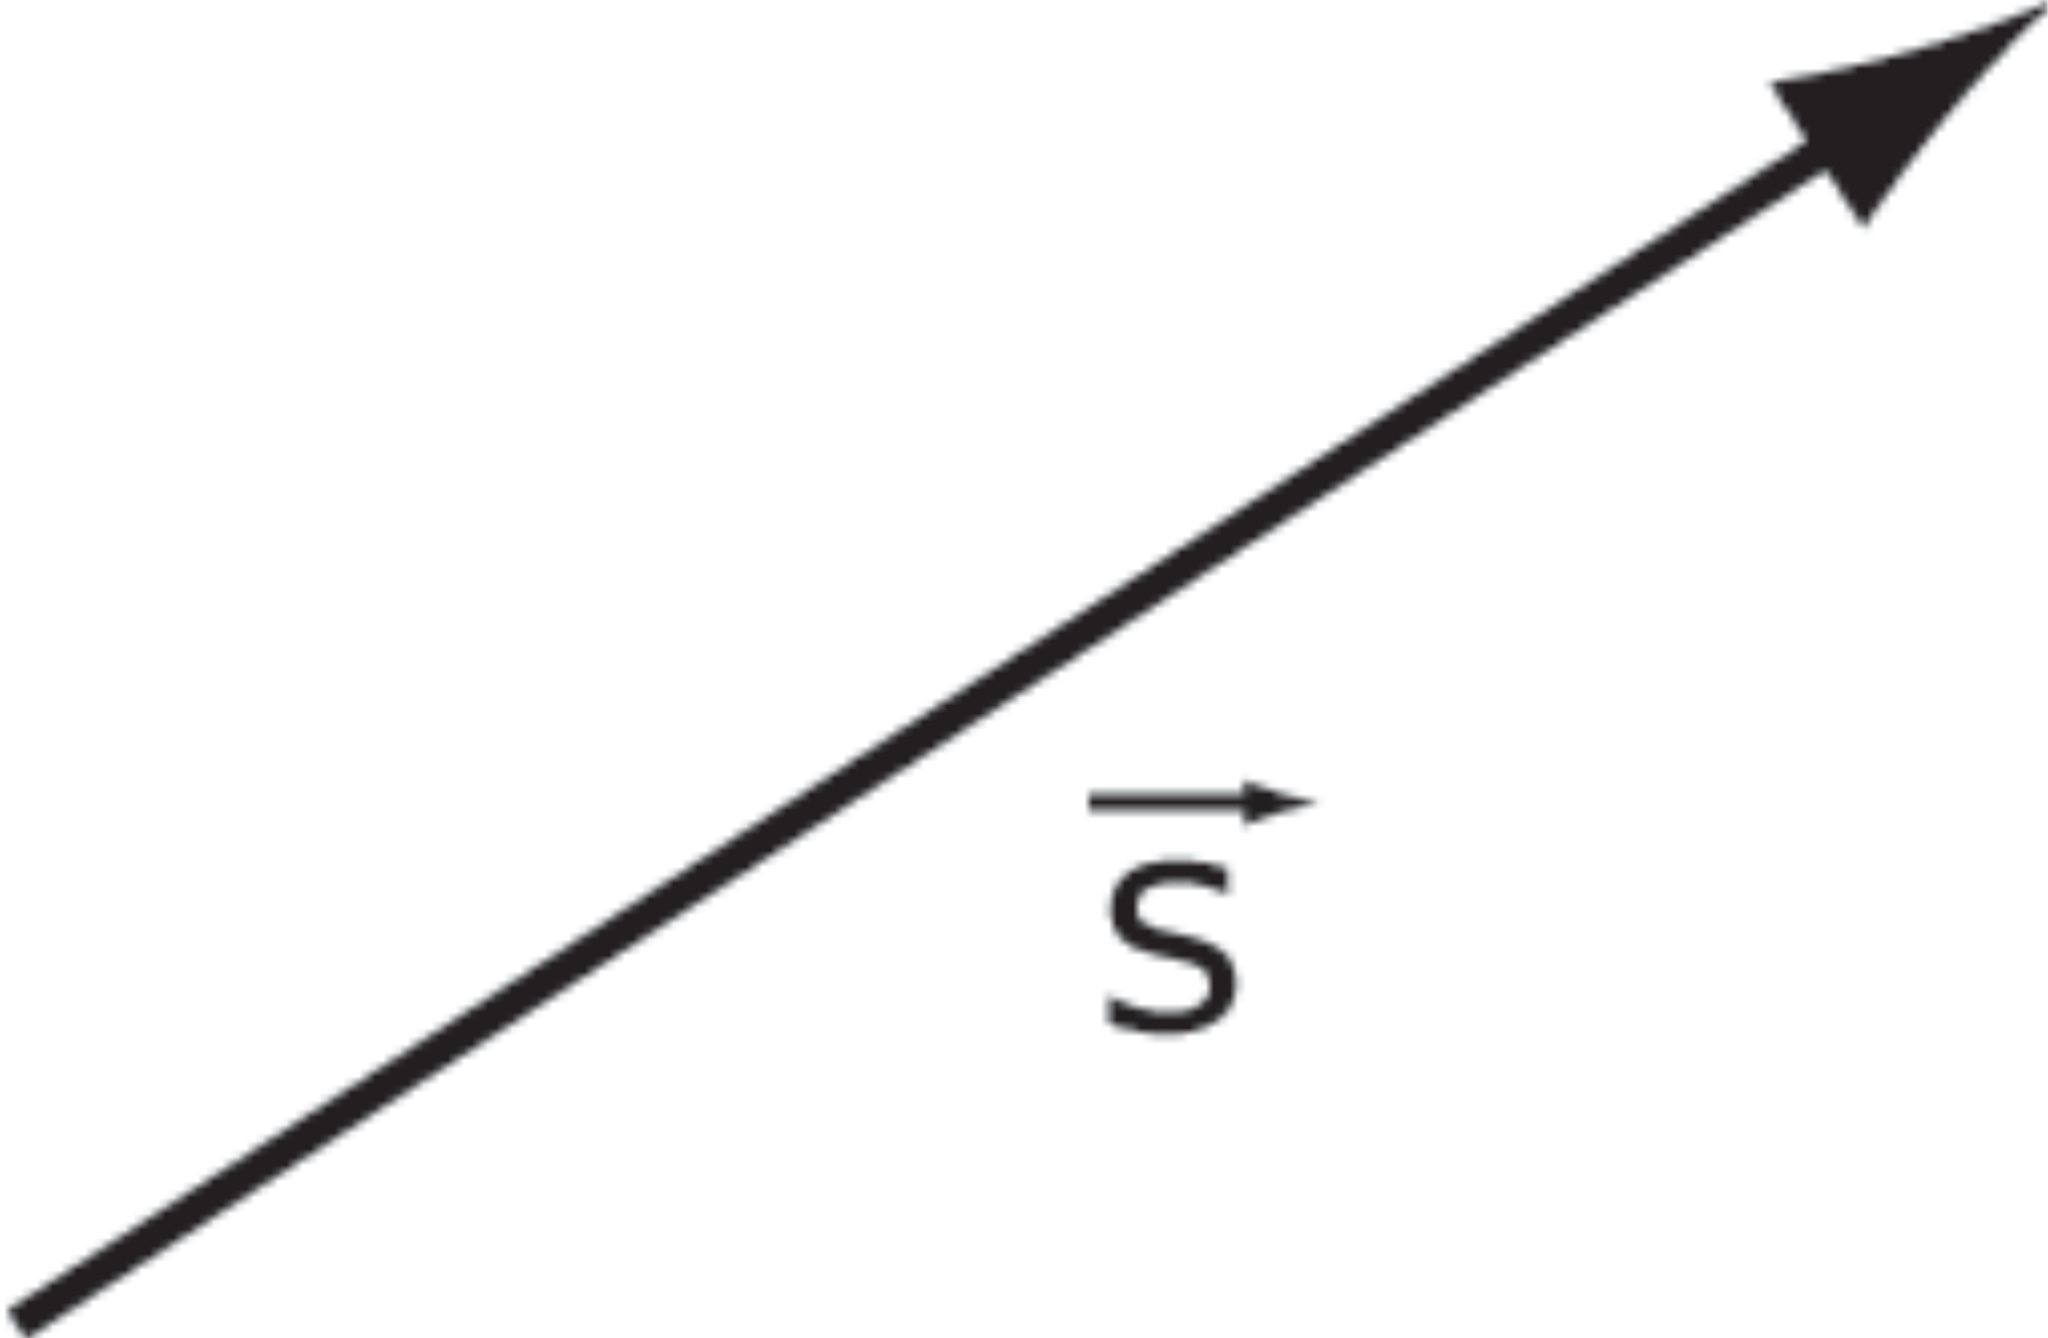
\includegraphics[width=2.3cm]{vecS} 
\scalebox{.8}{
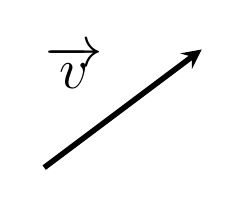
\begin{tikzpicture}
\begin{huge}
\draw [line width = 2pt,>=stealth,->] (0,0) -- (2,1.5) node[midway, above left] {$\overrightarrow{v}$};
\end{huge}
\end{tikzpicture}
} 
 \end{center}
 \end{minipage} \\
\end{aconnaitre}

\begin{remarque}
 Un vecteur peut avoir un nom, écrit avec une seule lettre en minuscule, par exemple $\overrightarrow{v}$ ou $\overrightarrow{s}$. Mais si la flèche qui représente le vecteur part d'un point $D$ et arrive au point $F$, alors on peut aussi appeler le vecteur $\overrightarrow{DF}$.
\end{remarque}


\begin{methode*1}[La translation]
\begin{exemple*1}
Construis l'image du triangle $ABC$ par la translation de vecteur $\vec{a}$ : \hfill
\begin{tabularx}{\linewidth}{X|X|X}
\textcolor{H1}{$\circled{1}$} & \textcolor{H1}{$\circled{2}$} & \textcolor{H1}{$\circled{3}$} \\
\scalebox{.4}{
\definecolor{CouleurPoints}{rgb}{0,0,1}
\begin{tikzpicture}[general,every node/.style={scale=2}]
%Les coordonnées du vecteur
\def \AbscVect {1};
\def \OrdVect {2};
%les sommets des 2 triangles 
\begin{huge}
\coordinate (A) at (3,1.6);
\coordinate (B) at (0,0);
\coordinate (C) at (4.5,-0.5);
%\coordinate (A') at (3+\AbscVect,1.6+\OrdVect);
%\coordinate (B') at (0+\AbscVect,0+\OrdVect);
%\coordinate (C') at (4.5+\AbscVect,-0.5+\OrdVect);
\draw[color=CouleurPoints] (A) node[right] {$A$};
\draw[color=CouleurPoints] (B) node[left] {$B$};
\draw[color=CouleurPoints] (C) node[right] {$C$};
%\draw[color=CouleurPoints] (A') node[right] {$A'$};
%\draw[color=CouleurPoints] (B') node[left] {$B'$};
%\draw[color=CouleurPoints] (C') node[right] {$C'$};

% les 3 cotés des triangles :
\draw[line width = 1.5pt] (A) -- (B) -- (C) -- cycle;
%\draw[line width = 0.4pt] (A') -- (B') -- (C') -- cycle;

%le vecteur de base
\draw [line width = 1.7pt,->] (5.4,0) -- ++(1,2) node[midway,below] {$\overrightarrow{a}$};

%les trois vecteurs partant des sommets
%\draw [>=stealth,->,line width = 1pt] (A) -- (A');
%\draw [>=stealth,->,line width = 1pt] (B) -- (B');
%\draw [>=stealth,->,line width = 1pt] (C) -- (C');

%les droites parallèles au vecteur
\draw[line width = 1.2pt] (A)-- ++(-1.3*\AbscVect,-1.3*\OrdVect) -- ++(2.5*\AbscVect,2.5*\OrdVect);
\draw[line width = 1.2pt] (B)-- ++(-0.5*\AbscVect,-0.5*\OrdVect) -- ++(2.5*\AbscVect,2.5*\OrdVect);
\draw[line width = 1.2pt] (C)-- ++(-0.5*\AbscVect,-0.5*\OrdVect) -- ++(2.5*\AbscVect,2.5*\OrdVect);
\end{huge}
\end{tikzpicture}
} 
 & \input{TranslationsRotations/figures/CoursMethode1_fig2.tex} & \input{TranslationsRotations/figures/CoursMethode1_fig3.tex} \\
\end{tabularx} \\
\textcolor{H1}{$\circled{1}$} On trace des droites parallèles au vecteur $\vec{a}$ passant par les sommets de la figure ;
\textcolor{H1}{$\circled{2}$} On reporte sur les droites le vecteur $\vec{a}$ en respectant le sens donné par la flèche ;
\textcolor{H1}{$\circled{3}$} On relie les sommets entre eux.
 \end{exemple*1}
 
 \begin{exemple*1}
$A'$ est l'image de $A$ par une translation. Construis l'image $B'$ de $B$ par cette translation :
\begin{tabularx}{\linewidth}{X|X|X}
\textcolor{H1}{$\circled{1}$} & \textcolor{H1}{$\circled{2}$} &\textcolor{H1}{$\circled{3}$} \\
\scalebox{.4}{
\begin{tikzpicture}[general,every node/.style={scale=2}]
%Les coordonnées du vecteur
\def \AbscVect {4};
\def \OrdVect {-2};
\begin{huge}
\coordinate (A) at (0,0);
\coordinate (B) at (7,2);
\coordinate (A') at (0+\AbscVect,0+\OrdVect);

\draw (A) node[above right] {$A$};
\draw (A) node{$\times$};
\draw (B) node[left] {$B$};
\draw (B) node{$\times$};
\draw (A') node[right] {$A'$};
\draw (A') node{$\times$};

\end{huge}
\end{tikzpicture}
} 
 & \scalebox{.4}{
\begin{tikzpicture}[general,every node/.style={scale=2}]
%Les coordonnées du vecteur
\def \AbscVect {4};
\def \OrdVect {-2};
\begin{huge}
\coordinate (A) at (0,0);
\coordinate (B) at (7,2);
\coordinate (A') at (0+\AbscVect,0+\OrdVect);

\draw (A) node[above right] {$A$};
\draw (A) node{$\times$};
\draw (B) node[left] {$B$};
\draw (B) node{$\times$};
\draw (A') node[right] {$A'$};
\draw (A') node{$\times$};

%le vecteur de base
\draw [line width = 2pt,>=stealth,->] (A) -- (A') node[midway, above right] {$\overrightarrow{AA'}$};

\end{huge}
\end{tikzpicture}
} 
  & \scalebox{.4}{
\begin{tikzpicture}[general,every node/.style={scale=2}]
%Les coordonnées du vecteur
\def \AbscVect {4};
\def \OrdVect {-2};
\begin{huge}
\coordinate (A) at (0,0);
\coordinate (B) at (7,2);
\coordinate (A') at (0+\AbscVect,0+\OrdVect);
\coordinate (B') at (7+\AbscVect,2+\OrdVect);
\draw (A) node[above right] {$A$};
\draw (A) node{$\times$};
\draw (B) node[left] {$B$};
\draw (B) node{$\times$};
\draw (A') node[right] {$A'$};
\draw (A') node{$\times$};
\draw (B') node[below left] {$B'$};
\draw (B') node{$\times$};

%le vecteur de base
\draw [line width = 2pt,>=stealth,->] (A) -- (A') node[midway, above right] {$\overrightarrow{AA'}$};
%\draw [line width = 2pt,>=stealth,->] (B) -- (B') node[midway, above right] {$\overrightarrow{BB'}$};
\end{huge}
\end{tikzpicture}
} 
\\ 
\end{tabularx} \\
\textcolor{H1}{$\circled{1}$} Les trois points sont donnés ;\\
\textcolor{H1}{$\circled{2}$} on trace d'abord le vecteur $\overrightarrow{AA'}$ ;\\
\textcolor{H1}{$\circled{2}$} on construit l'image du point $B$ par la translation de vecteur $\overrightarrow{AA'}$.
\end{exemple*1}

 \exercice
En t'aidant du quadrillage de ton cahier, reproduis la figure puis construis son imageS par la translation de vecteur $\overrightarrow{b}$ :
\begin{center} \includegraphics[width=4.5cm]{quadrillage_vecB} \end{center}
%\correction

 \end{methode*1}
 
%%%%%%%%%%%%%%%%%%%%%%%%%%%%%%%%%%%%%%%%%%%%%%%%%%%%%%%%%%%%%%%%%%%%%%%

\begin{aconnaitre}
Une \MotDefinition{rotation}{} est définie par son \textbf{centre} et son \textbf{angle}.

L'angle de rotation est \textbf{positif} si la rotation s'effectue dans le sens contraire des aiguilles d'une montre et \textbf{négatif} sinon.
\end{aconnaitre}

\begin{remarque}
La rotation de centre $O$ et d'angle $\alpha$ est notée : $R(O ; \alpha)$.
 \end{remarque}

\begin{methode*1}[La rotation]

 \begin{exemple*1}
 Construis l'image du triangle $ABC$ par la rotation $R(O ; - 45^\circ)$ :
 
%\begin{tabularx}{\linewidth}{X|X}
 %\textcolor{H1}{$\circled{1}$} & \textcolor{H1}{$\circled{2}$} \\
%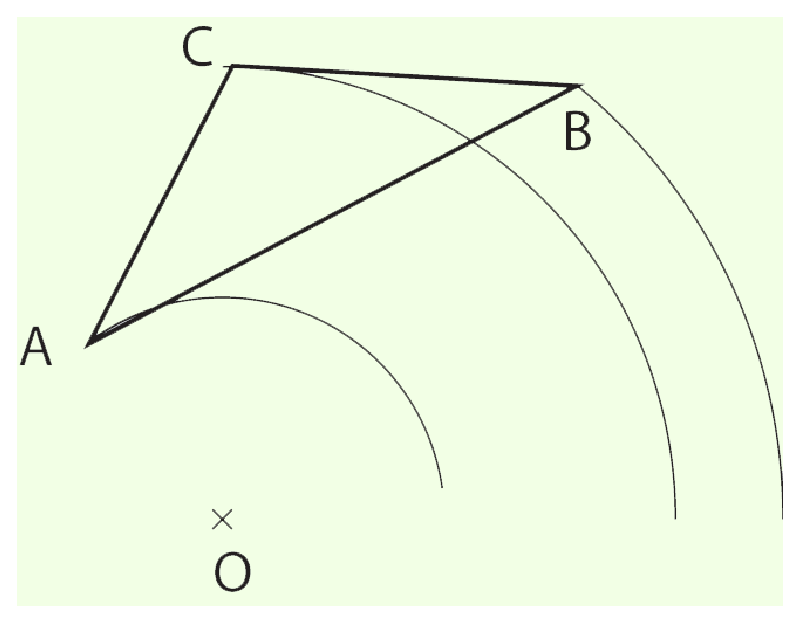
\includegraphics[width=4.7cm]{rotation_triangleABC} &  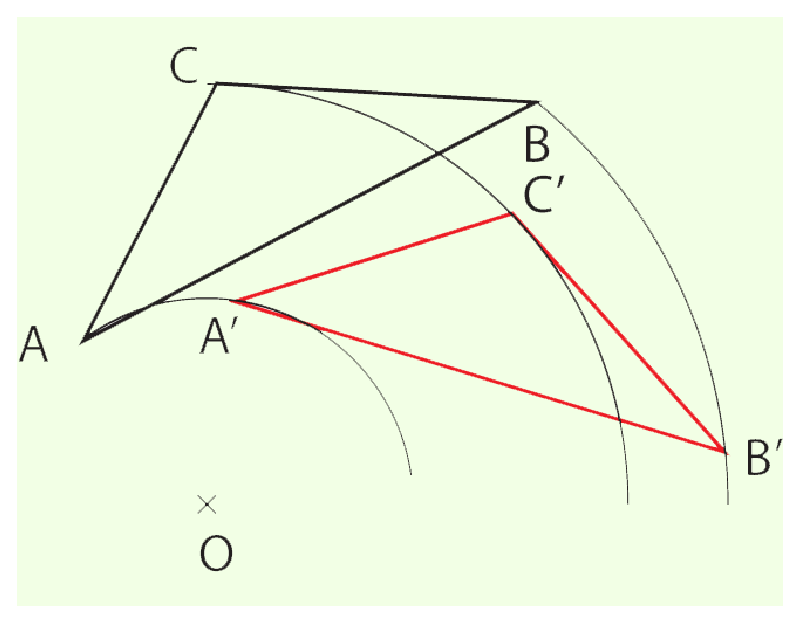
\includegraphics[width=4.7cm]{rotation_triangleABC2} \\ 
%\end{tabularx} \\

\textcolor{H1}{$\circled{1}$} La rotation s'effectue dans le sens des aiguilles d'une montre. On trace des arcs de cercles de centre $O$ passant par les sommets $A$, $B$ et $C$ ;
\textcolor{H1}{$\circled{2}$} On reporte l'angle de rotation sur tous les arcs de cercles ($\widehat{AOA'} = 45^\circ$) et on relie les sommets entre eux.
 \end{exemple*1}
 
\begin{exemple*1}
$A'$ et $B'$ sont l'image de $A$ et $B$ par une rotation. Détermine le centre de la rotation ainsi que l'angle de rotation :

\begin{minipage}[c]{0.44\linewidth}
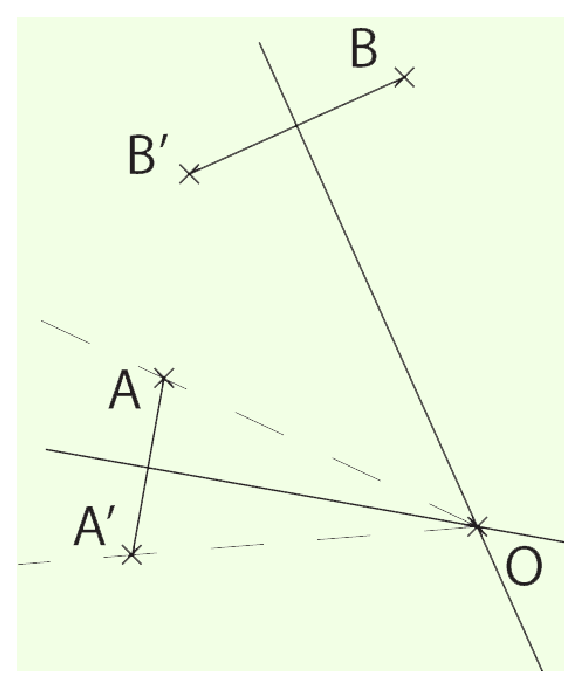
\includegraphics[width=3.7cm]{centre_rotation}
 \end{minipage} \hfill%
 \begin{minipage}[c]{0.52\linewidth}
On trace les médiatrices de $[AA']$ et $[BB']$. L'intersection des médiatrices donne le centre de la rotation $O$. \\[0.5em]
La rotation s'effectue dans le sens inverse des aiguilles d'une montre alors l'angle est positif. L'angle $\widehat{AOA'} = 30^\circ$ donc l'angle de rotation est $+ 30^\circ$
 \end{minipage} \\ 
 \end{exemple*1}

 \exercice
 En t'aidant du quadrillage de ton cahier, reproduis la figure puis construis son image par la rotation $R(O ; -90^\circ)$ : \\[0.5em]
 \begin{center} 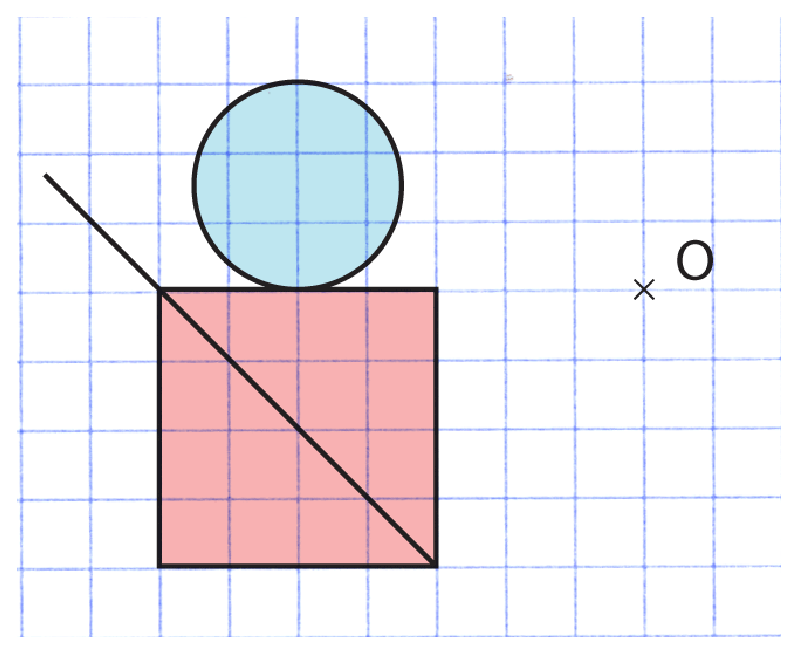
\includegraphics[width=5.2cm]{rotation_O60} \end{center}
%\correction

 \end{methode*1}
 
%%%%%%%%%%%%%%%%%%%%%%%%%%%%%%%%%%%%%%%%%%%%%%%%%%%%%%%%%%%%%%%%%%%%%%%


\exercicesbase
\begin{colonne*exercice}

\serie{Translation}

\begin{exercice}
Donne les cas où la transformation qui permet de passer de la figure 1 à la figure 2 est une translation :
\begin{center} \includegraphics[width=5.8cm]{translation_figures} \end{center}
\end{exercice}


\begin{exercice}
Quelles sont les cartes images de la carte $T$ par une translation ?
\begin{center} 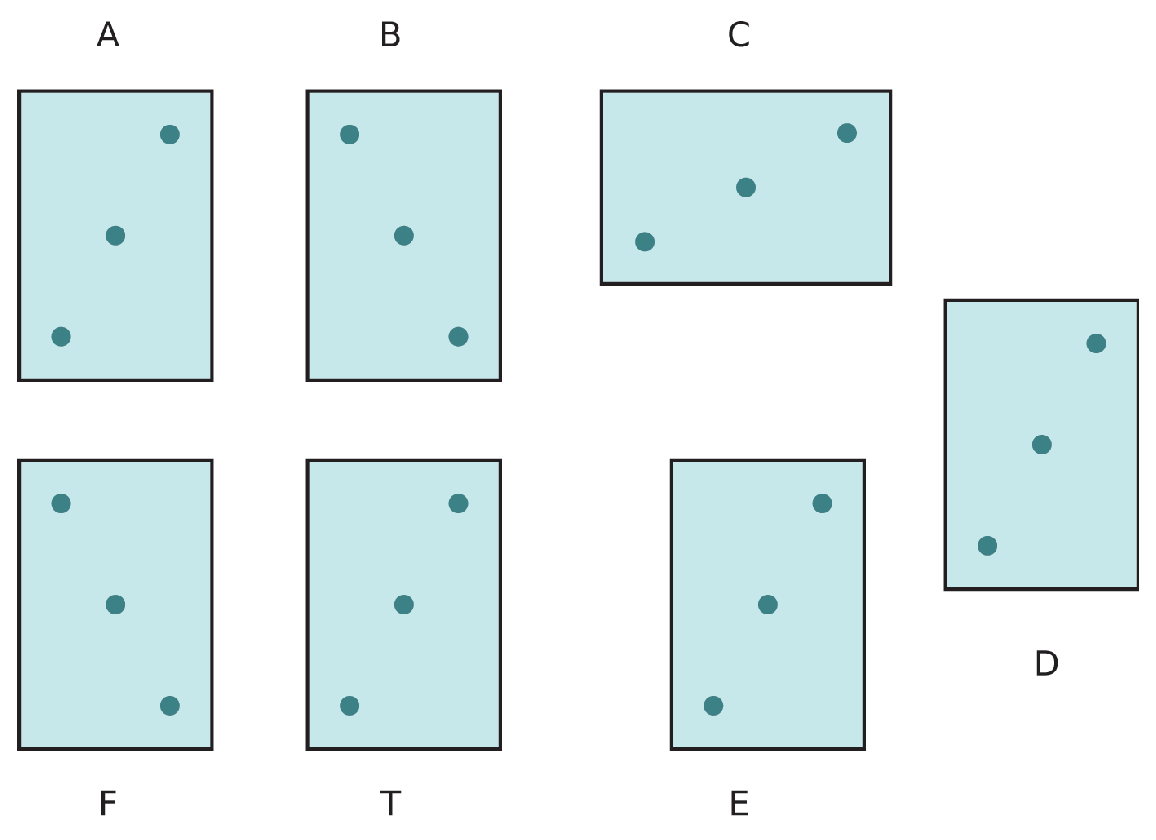
\includegraphics[width=8.1cm]{translation_cartes} \end{center}
\end{exercice}

%%%%%%%%%%%%%%%%%%%%%%%%%%%%%%%%%%%
%%%%%%%%%%%%%%%%%%%%%%%%%%%%%%%%%%%
%MiseEnPage
%%%%%%%%%%%%%%%%%%%%%%%%%%%%%%%%%%%
\columnbreak
%%%%%%%%%%%%%%%%%%%%%%%%%%%%%%%%%%%
%%%%%%%%%%%%%%%%%%%%%%%%%%%%%%%%%%%

\begin{exercice}
Complète les pointillés :
\begin{center} 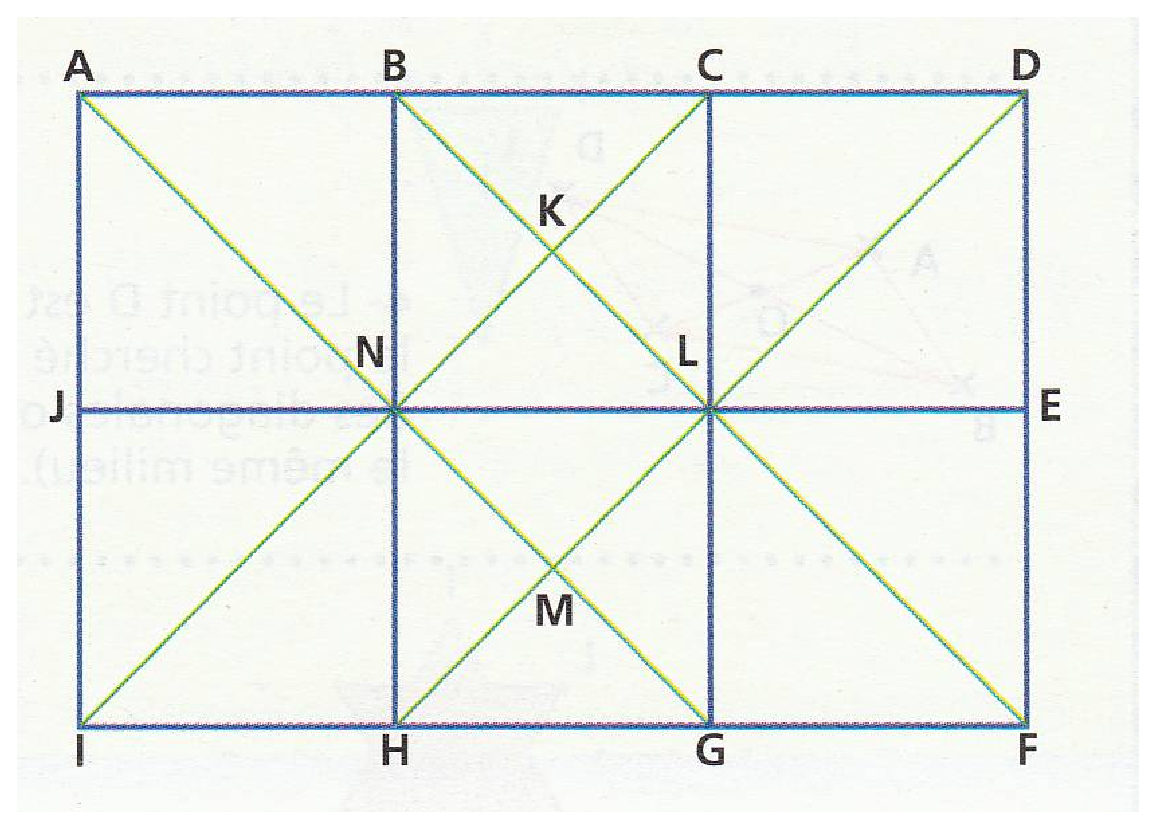
\includegraphics[width=4.5cm]{completer_translation} \end{center}
\begin{enumerate}
 \item L’image du point $L$ par la translation de vecteur $\overrightarrow{AB}$ est \ldots \ldots ;
 \item L’image du point \ldots \ldots par la translation de vecteur $\overrightarrow{BK}$ est $L$ ;
 \item L’image du point $J$ par la translation de vecteur \ldots \ldots est $L$ ;
 \item La translation de vecteur $\overrightarrow{DE}$, transforme $K$ en \ldots \ldots ;
 \item La translation qui transforme \ldots \ldots en $H$, transforme $N$ en $G$ ;
 \item Par la translation de vecteur $\overrightarrow{AJ}$, le triangle $BKN$ a pour image \ldots \ldots ;
 \item Par la translation de vecteur $\overrightarrow{JN}$, le triangle $NLH$ a pour image \ldots \ldots.
 \end{enumerate}
\end{exercice}


\begin{exercice}
Observe la figure ci-après puis recopie et complète dans ton cahier :
\begin{enumerate}
 \item Par la translation de vecteur $\overrightarrow{AC}$, l’image de la figure $\circled{2}$ est la figure \ldots ;
 \item Par la translation de vecteur $\overrightarrow{EC}$, l’image de la figure \ldots est la figure $\circled{2}$ ;
 \item Par la translation qui transforme \ldots en $C$, l’image de la figure $\circled{5}$ est la figure $\circled{6}$ ;
 \item La figure $\circled{3}$ est l’image de la figure \ldots par la translation de vecteur $\overrightarrow{CF}$ ;
 \item Dans la translation qui transforme $E$ en \ldots, l’image de la figure $\circled{3}$ est la figure $\circled{2}$.
 \end{enumerate}
\begin{center} 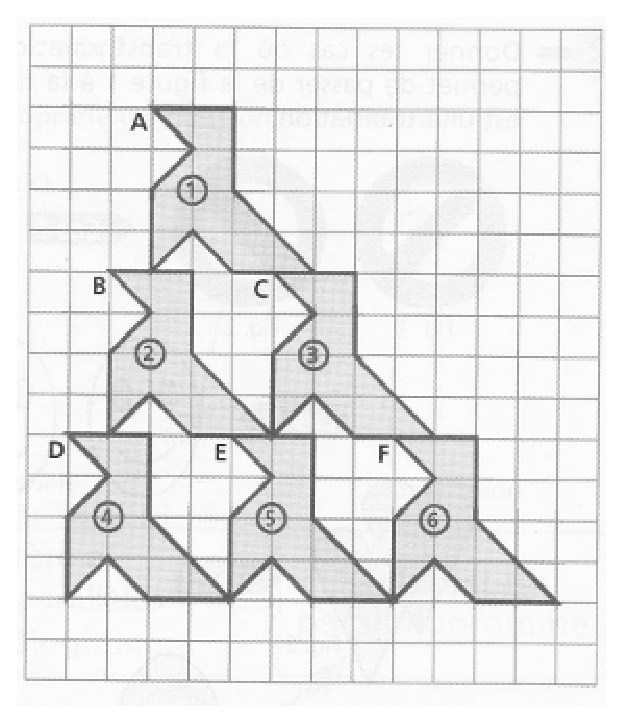
\includegraphics[width=4cm]{pyramide_jaune} \end{center}
\end{exercice}


\begin{exercice}
En t'aidant du quadrillage de ton cahier, recopie puis effectue la translation de vecteur $\vec{b}$ :
\begin{center} 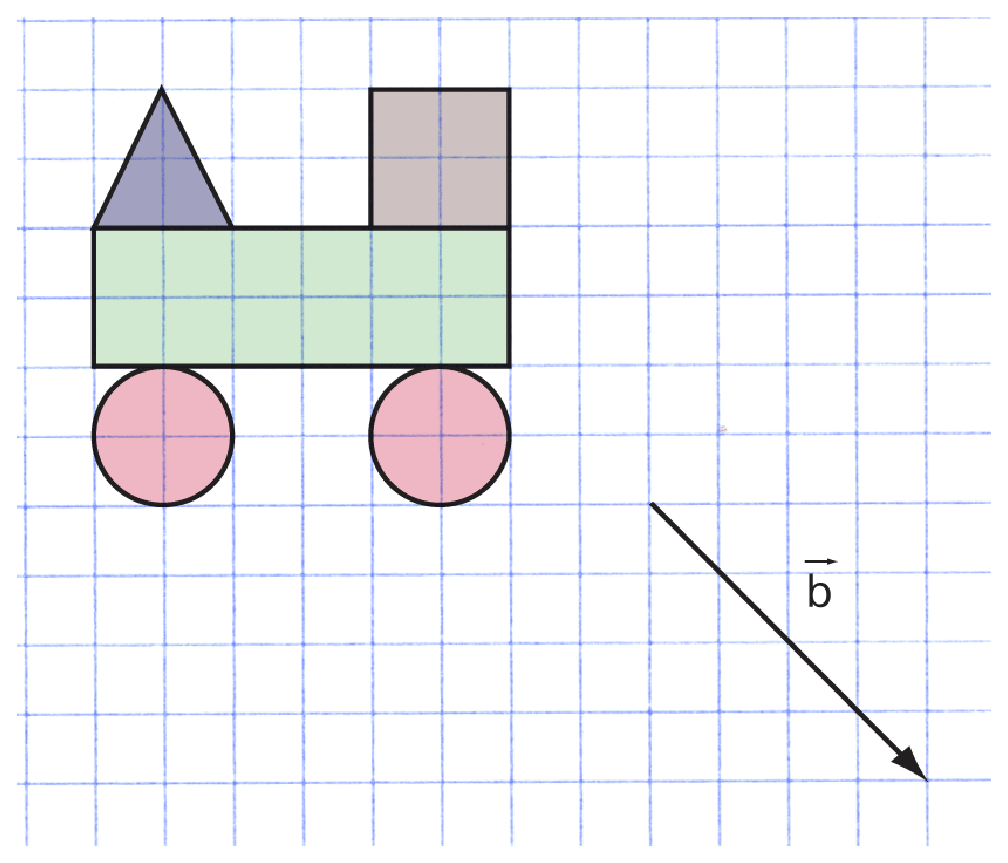
\includegraphics[width=5.4cm]{voiture_vecB} \end{center}
\end{exercice}


\begin{exercice}
En t'aidant du quadrillage de ton cahier, recopie puis effectue les translations :
\begin{center} 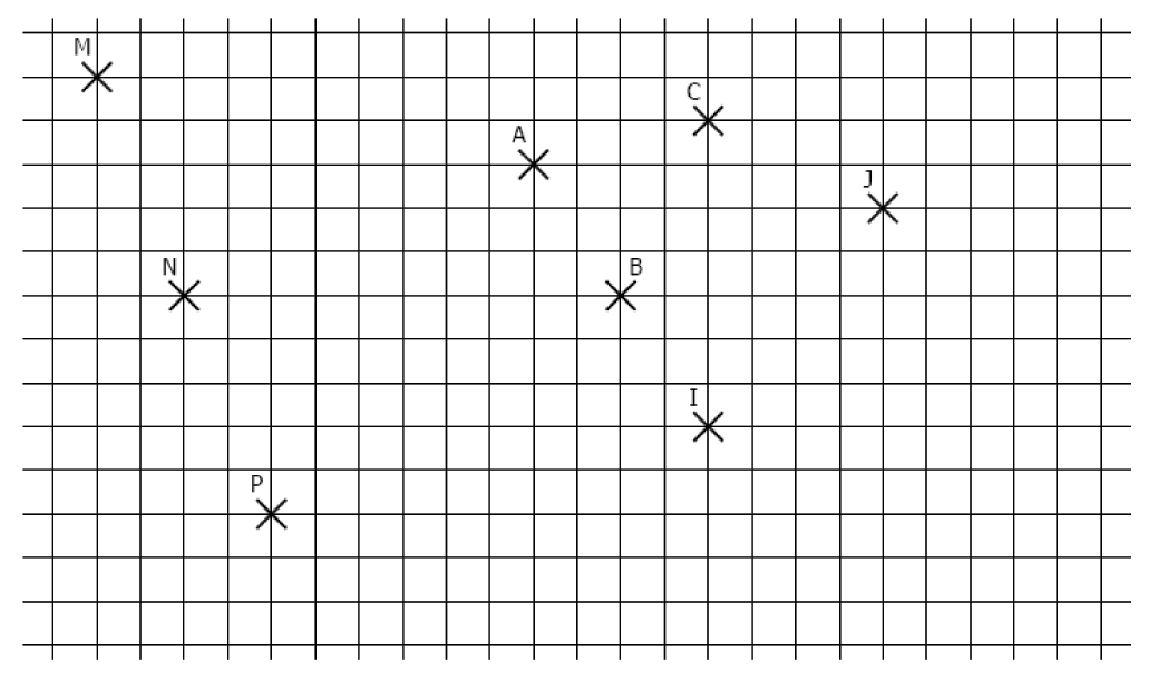
\includegraphics[width=8.1cm]{quadrillage_translations} \end{center}
\begin{enumerate}
 \item Construis le point $M_1$, image de $M$ par la translation de vecteur $\overrightarrow{AB}$ ;
 \item Construis le point $N_1$, image de $N$ par la translation de vecteur $\overrightarrow{AB}$ ;
 \item Construis le point $P_1$, image de $P$ par la translation de vecteur $\overrightarrow{AB}$ ;
 \item Construis le point $M_2$, image de $M$ par la translation de vecteur $\overrightarrow{AC}$ ;
 \item Construis le point $N_2$, image de $N$ par la translation de vecteur $\overrightarrow{AC}$ ;
 \item Construis le point $P_2$, image de $P$ par la translation de vecteur $\overrightarrow{AC}$ ;
 \item Construis le point $I_3$, image de $I$ par la translation de vecteur $\overrightarrow{MN}$ ;
 \item Construis le point $J_3$, image de $J$ par la translation de vecteur $\overrightarrow{MN}$ ;
 \item Construis le point $A_4$, image de $A$ par la translation de vecteur $\overrightarrow{BA}$ ;
 \item Construis le point $B_4$, image de $B$ par la translation de vecteur $\overrightarrow{BA}$.
 \end{enumerate}
\end{exercice}


\begin{exercice}
$[CD]$ est-il l'image de $[AB]$ par une translation ? Justifie ta réponse.
\begin{center} 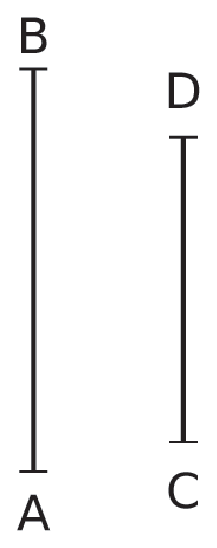
\includegraphics[width=1.2cm]{imageAB_CD} \end{center}
\end{exercice}


\begin{exercice}[Dans un repère]
Dans ton cahier trace un repère d'unité 1 cm pour chaque axe, puis place les points suivants : \\[0.5em]
\begin{tabular}{l|l}
$A(+ 3 ; + 2)$ \phantom{HELLO} & $D(+ 1 ; - 3)$ \\
$B(- 4 ; + 3)$ \phantom{HELLO} & $O(0 ; 0)$ \\
$C(- 2 ; - 1)$ \phantom{HELLO} & $T(+ 2 ; - 3)$ \\
 \end{tabular} \\

On considère la translation de vecteur $\overrightarrow{OT}$. Quelles sont les coordonnées des points $A'$, $B'$, $C'$, $D'$, images des points $A$, $B$, $C$, $D$ par cette translation.
\end{exercice}

%%%%%%%%%%%%%%%%%%%%%%%%%%%%%%%%%%%%%%%%%%%%%%%%%%%%%%%%%%%%%%%%%%%%%%%%%

\serie{Rotation}

\begin{exercice}
Détermine sur la figure ci-dessous quelles sont les images des points donnés par la rotation indiquée :
\begin{colenumerate}{2}
 \item $G$ par $R(O ; + 30^\circ)$ ;
 \item $T$ par $R(O ; + 60^\circ)$ ;
 \item $M$ par $R(O ; - 30^\circ)$ ;
 \item $I$ par $R(O ; - 60^\circ)$ ;
 \item $F$ par $R(O ; + 90^\circ)$ ;
 \item $G$ par $R(O ; - 120^\circ)$ ;
 \item $E$ par $R(O; + 120^\circ)$ ;
 \item $O$ par $R(O ; + 60^\circ)$ ;
 \item $E$ par $R(O ; + 180^\circ)$.
 \end{colenumerate}
\begin{center} 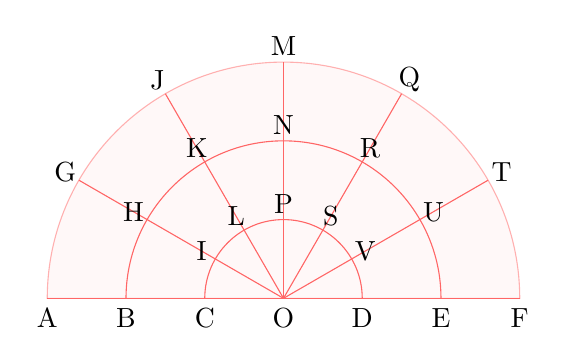
\begin{tikzpicture}	
  
    
\def \CharSize {1};
\def \BulletSize {1};


    %Définition de l 'angle de rotation de la figure
    \def \Rotation {0} 
    %Couleur des élèments de la figure (sauf le remplissage)
    \def \RapColor {red!60}


\begin{scope}[rotate=\Rotation]
    % contours
    \draw[color=\RapColor, fill =red!5, opacity=0.5] (-3,0) arc(180:0:3)--(3,0)--(-3,0)--cycle;	%Dont couleur de remplissage
    \draw[color=\RapColor] (-3,0)--(3,0);
    
   % demi-cercles intérieurs :
    \draw[color=\RapColor](-1,0) arc(180:0:1);
    \draw[color=\RapColor](-2,0) arc(180:0:2);
    
    
    % rayons :
   \foreach \a in {0,30,...,180}{\draw[color=\RapColor] (\a:3)--(\a:0);}
   
 
  
\end{scope}

\draw (0,0) node [below,scale=\CharSize]{O};
\draw (-3,0) node [below,scale=\CharSize]{A};
\draw (-2,0) node [below,scale=\CharSize]{B};
\draw (-1,0) node [below,scale=\CharSize]{C};
\draw (1,0) node [below,scale=\CharSize]{D};
\draw (2,0) node [below,scale=\CharSize]{E};
\draw (3,0) node [below,scale=\CharSize]{F};
\draw (150:3.2) node [scale=\CharSize]{G};
\draw (150:2.2) node [scale=\CharSize]{H};
\draw (150:1.2) node [scale=\CharSize]{I};
\draw (120:3.2) node [scale=\CharSize]{J};
\draw (120:2.2) node [scale=\CharSize]{K};
\draw (120:1.2) node [scale=\CharSize]{L};
\draw (90:3.2) node [scale=\CharSize]{M};
\draw (90:2.2) node [scale=\CharSize]{N};
\draw (90:1.2) node [scale=\CharSize]{P};
\draw (60:3.2) node [scale=\CharSize]{Q};
\draw (60:2.2) node [scale=\CharSize]{R};
\draw (60:1.2) node [scale=\CharSize]{S};
\draw (30:3.2) node [scale=\CharSize]{T};
\draw (30:2.2) node [scale=\CharSize]{U};
\draw (30:1.2) node [scale=\CharSize]{V};
    
\end{tikzpicture} 
 \end{center}
\end{exercice}

%%%%%%%%%%%%%%%%%%%%%%%%%%%%%%%%%%%
%%%%%%%%%%%%%%%%%%%%%%%%%%%%%%%%%%%
%MiseEnPage
%%%%%%%%%%%%%%%%%%%%%%%%%%%%%%%%%%%
\newpage
%%%%%%%%%%%%%%%%%%%%%%%%%%%%%%%%%%%
%%%%%%%%%%%%%%%%%%%%%%%%%%%%%%%%%%%

\vspace{-2.5cm}
\begin{exercice}
Détermine sur la figure ci-dessous, l'angle de la rotation de centre $O$ telle que l'image de \ldots
\begin{colenumerate}{3}
 \item $M$ donne $J$ ;
 \item $U$ donne $N$ ;
 \item $K$ donne $N$ ;
 \item $P$ donne $V$ ;
 \item $D$ donne $I$ ;
 \item $H$ donne $U$ ;
 \item $B$ donne $U$ ;
 \item $F$ donne $A$ ;
 \item $I$ donne $S$.
 \end{colenumerate}
\begin{center} 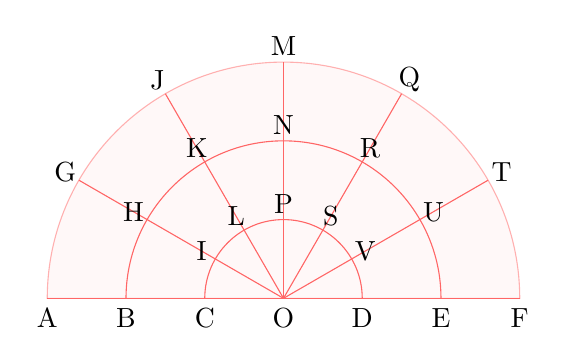
\begin{tikzpicture}	
  
    
\def \CharSize {1};
\def \BulletSize {1};


    %Définition de l 'angle de rotation de la figure
    \def \Rotation {0} 
    %Couleur des élèments de la figure (sauf le remplissage)
    \def \RapColor {red!60}


\begin{scope}[rotate=\Rotation]
    % contours
    \draw[color=\RapColor, fill =red!5, opacity=0.5] (-3,0) arc(180:0:3)--(3,0)--(-3,0)--cycle;	%Dont couleur de remplissage
    \draw[color=\RapColor] (-3,0)--(3,0);
    
   % demi-cercles intérieurs :
    \draw[color=\RapColor](-1,0) arc(180:0:1);
    \draw[color=\RapColor](-2,0) arc(180:0:2);
    
    
    % rayons :
   \foreach \a in {0,30,...,180}{\draw[color=\RapColor] (\a:3)--(\a:0);}
   
 
  
\end{scope}

\draw (0,0) node [below,scale=\CharSize]{O};
\draw (-3,0) node [below,scale=\CharSize]{A};
\draw (-2,0) node [below,scale=\CharSize]{B};
\draw (-1,0) node [below,scale=\CharSize]{C};
\draw (1,0) node [below,scale=\CharSize]{D};
\draw (2,0) node [below,scale=\CharSize]{E};
\draw (3,0) node [below,scale=\CharSize]{F};
\draw (150:3.2) node [scale=\CharSize]{G};
\draw (150:2.2) node [scale=\CharSize]{H};
\draw (150:1.2) node [scale=\CharSize]{I};
\draw (120:3.2) node [scale=\CharSize]{J};
\draw (120:2.2) node [scale=\CharSize]{K};
\draw (120:1.2) node [scale=\CharSize]{L};
\draw (90:3.2) node [scale=\CharSize]{M};
\draw (90:2.2) node [scale=\CharSize]{N};
\draw (90:1.2) node [scale=\CharSize]{P};
\draw (60:3.2) node [scale=\CharSize]{Q};
\draw (60:2.2) node [scale=\CharSize]{R};
\draw (60:1.2) node [scale=\CharSize]{S};
\draw (30:3.2) node [scale=\CharSize]{T};
\draw (30:2.2) node [scale=\CharSize]{U};
\draw (30:1.2) node [scale=\CharSize]{V};
    
\end{tikzpicture} 
 \end{center}
\end{exercice}


\begin{exercice}
En t'aidant du quadrillage de ton cahier reporte les points suivants :
\begin{center} 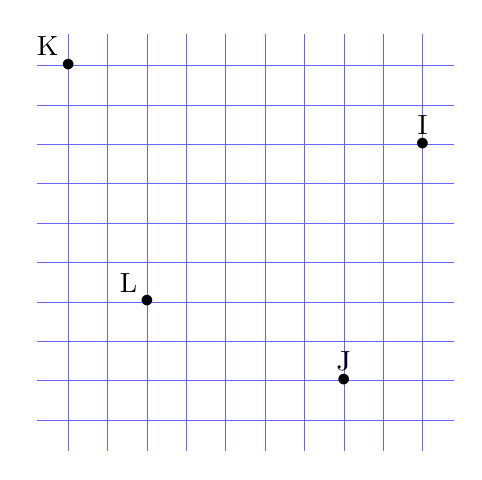
\begin{tikzpicture}	
  
    
\def \CharSize {1};
\def \BulletSize {1};


\draw[very thin, blue!60] (0.1,-0.9) grid[step=0.5] (5.4,4.4);

\draw (0.5,4) node [above left,scale=\CharSize]{K};
\draw (0.5,4) node[scale=\BulletSize]{$\bullet$};
\draw (1.5,1) node [above left,scale=\CharSize]{L};
\draw (1.5,1) node[scale=\BulletSize]{$\bullet$};
\draw (5,3) node [above,scale=\CharSize]{I};
\draw (5,3) node[scale=\BulletSize]{$\bullet$};
\draw (4,0) node [above,scale=\CharSize]{J};
\draw (4,0) node[scale=\BulletSize]{$\bullet$};
\end{tikzpicture}  \end{center}
Construis le point :
\begin{enumerate}
 \item $J_1$ image de $J$ par la rotation de centre $I$ et d’angle $+ 90^\circ$ ;
 \item $K_1$ image de $K$ par la rotation de centre $I$ et d’angle $- 90^\circ$ ;
 \item $L_1$ image de $L$ par la rotation de centre $I$ et d’angle $+ 90^\circ$ ;
 \item $I_2$ image de $I$ par la rotation de centre $K$ et d’angle $- 45^\circ$ ;
 \item $J_2$ image de $J$ par la rotation de centre $K$ et d’angle $+ 45^\circ$ ;
 \item $L_2$ image de $L$ par la rotation de centre $K$ et d’angle $- 45^\circ$.
 \end{enumerate}
\end{exercice}


\begin{exercice}
Reproduis la lettre $F$ dans ton cahier. Construis l'image la lettre $F$ par la rotation de centre $O$, d'angle $+ 90^\circ$.
\begin{center} 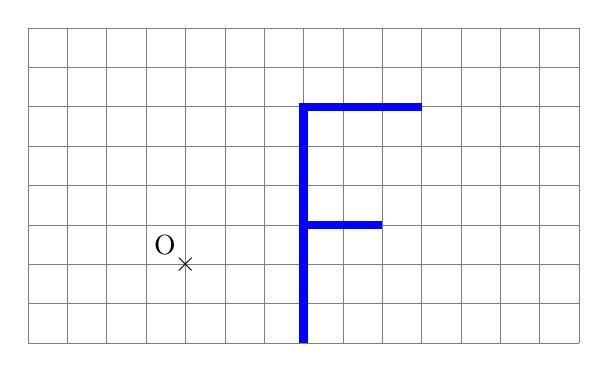
\begin{tikzpicture}	
  
    
\def \CharSize {1};
\def \BulletSize {1};


\draw[very thin, gray] (0,0) grid[step=0.5] (7,4);

\draw (2,1) node [above left,scale=\CharSize]{O};
\draw (2,1) node[thick,scale=\BulletSize]{$\times$};
\draw[line width=3pt,blue] (3.5,0)--(3.5,3)--(5,3);
\draw[line width=3pt,blue] (3.5,1.5)--(4.5,1.5);

\end{tikzpicture}  \end{center}
\end{exercice}


\begin{exercice}
Reproduis la lettre $E$ dans ton cahier. Construis l'image de lettre $E$ par la rotation de centre $O$, d'angle $- 45^\circ$.
\begin{center} 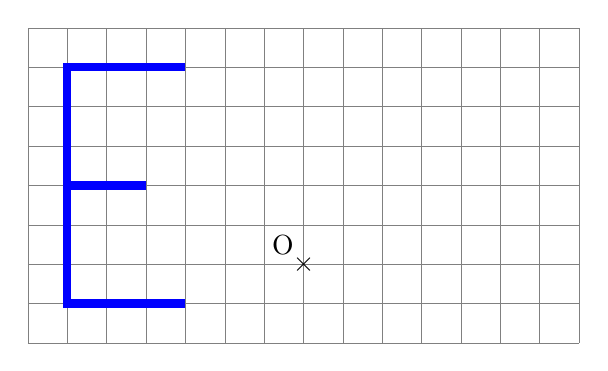
\begin{tikzpicture}	
  
    
\def \CharSize {1};
\def \BulletSize {1};


\draw[very thin, gray] (0,0) grid[step=0.5] (7,4);

\draw (3.5,1) node [above left,scale=\CharSize]{O};
\draw (3.5,1) node[thick,scale=\BulletSize]{$\times$};
\draw[line width=3pt,blue] (2,0.5)--(0.5,0.5)--(0.5,3.5)--(2,3.5);
\draw[line width=3pt,blue] (0.5,2)--(1.5,2);

\end{tikzpicture} 
 \end{center}
\end{exercice}


\begin{exercice}
Soit $ABC$ un triangle tel que $\widehat{BAC}$ mesure $60^\circ$; $[AB]$ mesure 4cm et $[AC]$ mesure 3cm. Soit $O$ un point extérieur au triangle $ABC$.
\begin{enumerate}
 \item Faire une figure sur une feuille blanche ;
 \item Construire le triangle $A'B'C'$ image du triangle $ABC$ par la rotation de centre $O$, d'angle $+ 40^\circ$.
 \end{enumerate}
\end{exercice}


\begin{exercice}
Soit $A$ et $B$ deux point distincts. Soit $E$ l'image de $B$ par la rotation de centre $A$, d'angle $+ 30^\circ$. Soit $F$ l'image de $B$ par la rotation de centre $A$, d'angle $- 60^\circ$.
\begin{enumerate}
 \item Trace la figure.
 \item Quelle est la nature du triangle $AEF$ ?
 \end{enumerate}
\end{exercice}

\end{colonne*exercice}


\exercicesappr
\begin{colonne*exercice}
\begin{exercice}[Tangram]
Le Tangram est découpé dans un carré. Il est formé de 5 triangles rectangles isocèles, les pièces $\circled{1}$, $\circled{2}$, $\circled{3}$, $\circled{4}$, $\circled{5}$, d'un parallélogramme $\circled{6}$ et d'un carré $\circled{7}$ :
%\begin{center} \includegraphics[width=5.2cm]{tangram} \end{center}

En observant le dessin de ce puzzle, réponds aux questions suivantes :
\begin{enumerate}
 \item Quelle est l'image de $H$ par la translation $\overrightarrow{FB}$ ?
 \item Quelle est l'image de $I$ par la rotation de centre $J$, d'angle $90^\circ$ ?
 \item Quelle est l'image de $H$ par la translation $\overrightarrow{GF}$ suivie de la translation $\overrightarrow{BF}$ ?
 \item Quelle est l'image de $B$ par la symétrie de centre $F$ ?
 \item Quelle est l'image de $A$ par la symétrie d'axe $(BD)$ ?
 \item Quelle est l'image de $J$ par la symétrie de centre $G$ suivie de la symétrie de centre $H$ ?
 \end{enumerate}
\end{exercice}


\begin{exercice}[En repérage]
Dans un repère d'unité 1 cm pour chaque axe, on effectue une translation donnée par le point $A(2 ; 5)$ et son image $A'(5 ; 8)$.
\begin{enumerate}
 \item Quelles sont les coordonnées des images des points $B(5 ; - 1)$, $C(- 4 ; - 2)$ et $D(- 4 ; 2)$ ?
 \item Quelles sont les coordonnées des points dont les images sont $E'(- 2 ; - 3)$, $F'(3 ; 5)$ et $G'(0 ; 0)$ ?
 \end{enumerate}
\end{exercice}


\begin{exercice}[Doublé gagnant]
Dans un repère d'unité 1 cm pour chaque axe, l'image du triangle $ABC$ par la translation $\vec{T_1}$ est le triangle $A'B'C'$. L'image du triangle $A'B'C'$ par la translation $\vec{T_2}$ est le triangle $A''B''C''$. \\[0.5em]
Construis les trois triangles $ABC$, $A'B'C'$ et $A''B''C''$ connaissant les points $A(6 ; 4)$, $C(16 ; 2)$, $B'(- 8 ; - 3)$, $C'(- 8 ; - 6)$,et $B''(6 ; - 8)$.
\end{exercice}


\begin{exercice}[À condition]
\begin{enumerate}
 \item Soit $[AB]$ et $[A'B']$ deux segments isométriques. À quelle(s) condition(s) existe-t-il une translation qui associe $[AB]$ à $[A'B']$ ?
 \item À quelle(s) condition(s) deux cercles $C$ et $C'$ sont-ils images l'un de l'autre par une translation ?
 \end{enumerate}
\end{exercice}



\end{colonne*exercice}

\connaissances

\QCMautoevaluation{Pour chaque question, plusieurs réponses sont
  proposées.  Déterminer celles qui sont correctes.}

\begin{QCM}
  \begin{GroupeQCM}
    \begin{exercice}
       \begin{center} \scalebox{1}{

\begin{tikzpicture}[general]

\draw (-1,-1) node[below] {$A$};
\draw (0,-1) node[below] {$B$};
\draw (0,0) node[below right] {$C$};
\draw (-1,0) node[above] {$D$};
\draw (0,0) node[above left] {$A'$};
\draw (1,0) node[right] {$B'$};
\draw (1,1) node[above right] {$C'$};
\draw (0,1) node[above] {$D'$};

\draw[line width = 1.5pt] (-1,-1) -- (0,-1) -- (0,0) -- (-1,0) -- cycle;
\draw[line width = 1.5pt] (0,0) -- (1,0) -- (1,1) -- (0,1) -- cycle;

\end{tikzpicture}
}
 \end{center}
       Le carré $A'B'C'D'$ est l'image du carré $ABCD$ par la translation de vecteur \ldots
      \begin{ChoixQCM}{4}
      \item $\overrightarrow{AB}$
      \item $\overrightarrow{AC}$
      \item $\overrightarrow{AD}$
      \item $\overrightarrow{BD}$
      \end{ChoixQCM}
\begin{corrige}
     \reponseQCM{b}
   \end{corrige}
    \end{exercice}
    
    
    \begin{exercice}
         \begin{center} 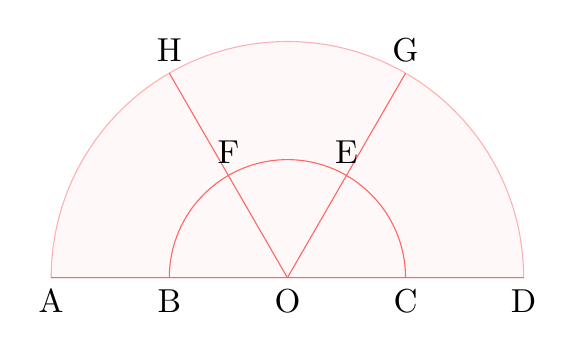
\begin{tikzpicture}	
  
    
\def \CharSize {1.2};
\def \BulletSize {1};


    %Définition de l 'angle de rotation de la figure
    \def \Rotation {0} 
    %Couleur des élèments de la figure (sauf le remplissage)
    \def \RapColor {red!60}


\begin{scope}[rotate=\Rotation]
    % contours
    \draw[color=\RapColor, fill =red!5, opacity=0.5] (-3,0) arc(180:0:3)--(3,0)--(-3,0)--cycle;	%Dont couleur de remplissage
    \draw[color=\RapColor] (-3,0)--(3,0);
    
   % demi-cercle intérieur :
    \draw[color=\RapColor](-1.5,0) arc(180:0:1.5);
    
    % rayons :
   \foreach \a in {0,60,...,180}{\draw[color=\RapColor] (\a:3)--(\a:0);}
   
 
  
\end{scope}

\draw (0,0) node [below,scale=\CharSize]{O};
\draw (1.5,0) node [below,scale=\CharSize]{C};
\draw (3,0) node [below,scale=\CharSize]{D};
\draw (-1.5,0) node [below,scale=\CharSize]{B};
\draw (-3,0) node [below,scale=\CharSize]{A};
\draw (60:1.5) node [above,scale=\CharSize]{E};
\draw (120:1.5) node [above,scale=\CharSize]{F};
\draw (60:3) node [above,scale=\CharSize]{G};
\draw (120:3) node [above,scale=\CharSize]{H};
    
\end{tikzpicture} 
  \end{center}
      $E$ est l'image de $F$ par la rotation de centre $O$ et d'angle \ldots
      \begin{ChoixQCM}{4}
      \item $+ 30^\circ$
      \item $- 30^\circ$
      \item $+ 60^\circ$
      \item $- 60^\circ$
      \end{ChoixQCM}
\begin{corrige}
     \reponseQCM{d}
   \end{corrige}
    \end{exercice}
    
    
    \begin{exercice}
      Sur l'image ci-dessus, l'image de $D$ par une rotation de centre $O$ et d'angle $120^\circ$ est \ldots
      \begin{ChoixQCM}{4}
      \item $A$
      \item $H$
      \item $G$
      \item $O$
      \end{ChoixQCM}
\begin{corrige}
     \reponseQCM{b}
   \end{corrige}
    \end{exercice}


\end{GroupeQCM}
\end{QCM}

  


\TravauxPratiques % pour nous "travailler en groupe"

\begin{TP}[Figure de Kolam]

\begin{minipage}[t]{0.48\linewidth}
Dans l'État du Tamil Nadu, dans le sud-est de l'Inde, les mères enseignent à leurs filles l'art de dessiner avec de la poudre de riz des figures de Kolam qui décorent le seuil des habitations.
 \end{minipage} \hfill%
 \begin{minipage}[t]{0.48\linewidth}
 \begin{enumerate}
  \item Sur une feuille blanche, reproduisez la figure $A$ ;
  \item Complétez la figure $A$ afin d'obtenir la figure $B$ en effectuant des rotations. Trouvez le centre des rotations ;
  \item Complétez la figure pour obtenir la figure C. 
  \end{enumerate}
  \end{minipage} \\
  
\begin{minipage}[t]{0.32\linewidth}
 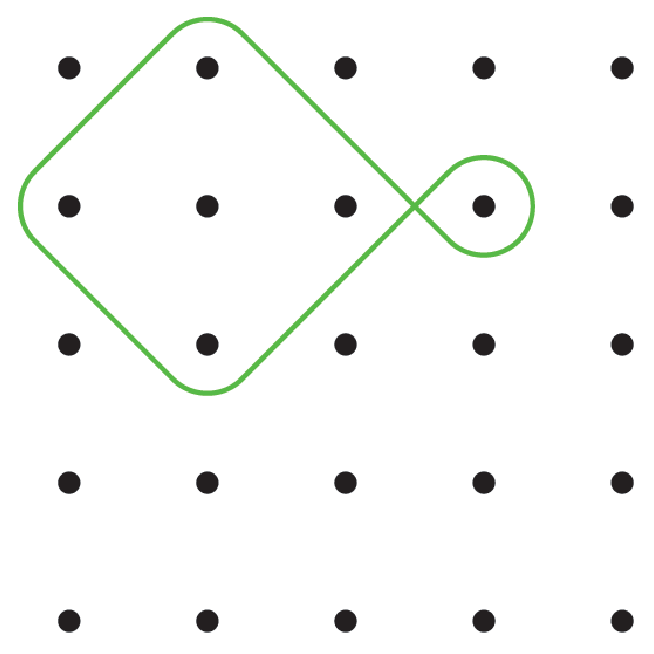
\includegraphics[width=3.6cm]{Kolam1}
 \end{minipage} \hfill%
 \begin{minipage}[t]{0.32\linewidth}
  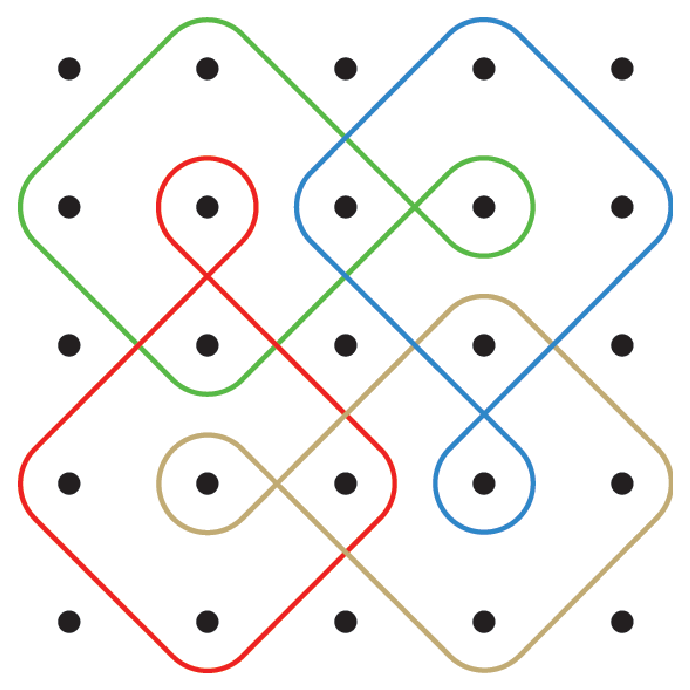
\includegraphics[width=3.6cm]{Kolam2}
  \end{minipage} \hfill%
  \begin{minipage}[t]{0.32\linewidth}
   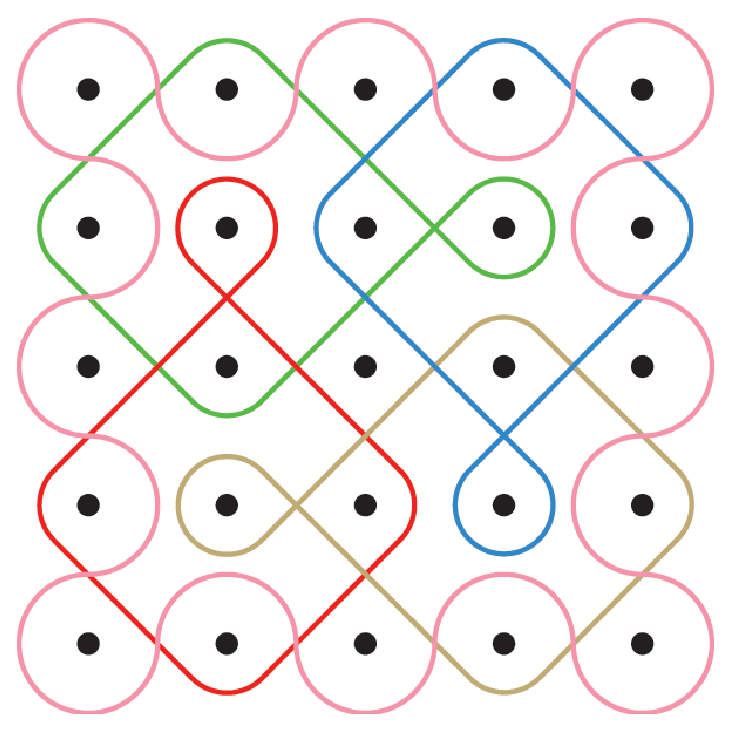
\includegraphics[width=3.6cm]{Kolam3}
   \end{minipage} \\

\end{TP}

%%%%%%%%%%%%%%%%%%%%%%%%%%%%%%%%%%%
%%%%%%%%%%%%%%%%%%%%%%%%%%%%%%%%%%%
%MiseEnPage
%%%%%%%%%%%%%%%%%%%%%%%%%%%%%%%%%%%
\vfill
%%%%%%%%%%%%%%%%%%%%%%%%%%%%%%%%%%%
%%%%%%%%%%%%%%%%%%%%%%%%%%%%%%%%%%%


\pagebreak

\recreation
\begin{enigme}[La dalle (d’après le GVJM)]

Dans un jardin carré de 10 m de côté, Maurice tend une corde entre chaque coin et le milieu du côté opposé, comme indiqué sur la figure. Les quatre cordes ainsi tendues délimitent une surface à l’intérieur de laquelle des ouvriers coulent une dalle en ciment (partie ombrée). Quelle est l’aire de cette dalle ? \\[0.5em]
Indice : fais pivoter certains triangles.
\begin{center} 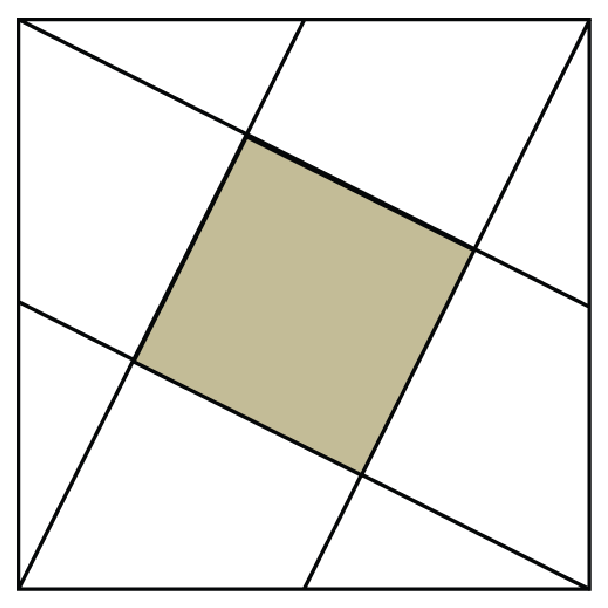
\includegraphics[width=4.7cm]{dalleGVJM} \end{center}
\end{enigme} 

%%%%%%%%%%%%%%%%%%%%%%%%%%%%%%%%%%%%%%%%%%%%%%%%%%%%%%%%%%%%%%%%%%%%%%%%%

\begin{enigme}[La disparition (d’après le GVJM)]

Construis 7 bâtonnets de 2 cm de hauteur et distants chacun de 1 cm, selon le croquis ci-dessous. Trace une ligne comme indiqué, du bas du premier bâtonnet au haut du dernier. Coupe ta figure en deux, le long de la ligne tracée. En translatant la partie du haut contre la partie du bas le long de la ligne de coupe, tu peux faire disparaître un bâtonnet. \\[0.5em]
Comment expliques-tu ce tour de magie ?
\begin{center} 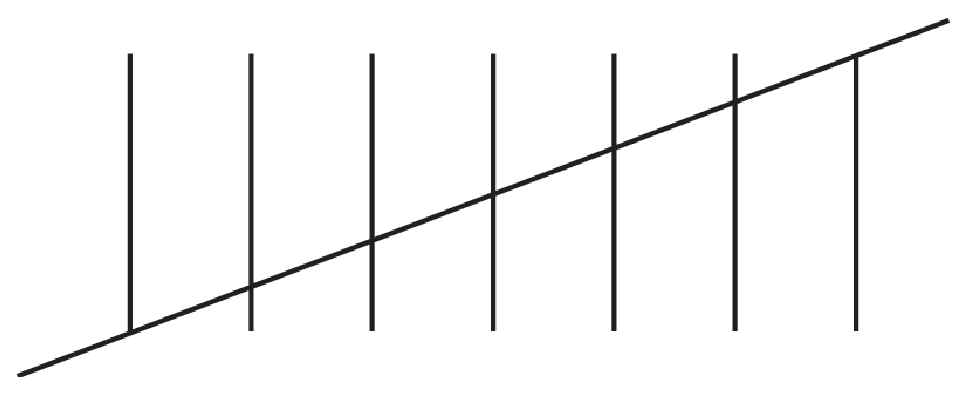
\includegraphics[width=7.5cm]{dalle_magie} \end{center}
\end{enigme} 


